\documentclass[a4paper,10pt]{article}

\usepackage[brazilian]{babel}
\usepackage[left=2.5cm,right=2.5cm,top=3cm,bottom=2.5cm]{geometry}
\usepackage{mathtools}
\usepackage{amsthm}
\usepackage{amsmath}
%\usepackage{nccmath}
\usepackage{amssymb}
\usepackage{amsfonts}
\usepackage{physics}
%\usepackage{dsfont}
%\usepackage{mathrsfs}

\usepackage{titling}
\usepackage{indentfirst}

\usepackage{bm}
\usepackage[dvipsnames]{xcolor}
\usepackage{cancel}

\usepackage{xurl}
\usepackage[colorlinks=true]{hyperref}

\usepackage{float}
\usepackage{graphicx}
%\usepackage{tikz}
\usepackage{caption}
\usepackage{subcaption}

%%%%%%%%%%%%%%%%%%%%%%%%%%%%%%%%%%%%%%%%%%%%%%%%%%%

\newcommand{\eps}{\epsilon}
\newcommand{\vphi}{\varphi}
\newcommand{\cte}{\text{cte}}

\newcommand{\N}{\mathbb{N}}
\newcommand{\Z}{\mathbb{Z}}
\newcommand{\Q}{\mathbb{Q}}
\newcommand{\R}{\vb{R}}
\newcommand{\C}{\mathbb{C}}
\renewcommand{\S}{\hat{S}}
%\renewcommand{\H}{\s{H}}

\renewcommand{\a}{\vb{a}}
\newcommand{\nn}{\hat{n}}
\renewcommand{\d}{\dagger}
\newcommand{\up}{\uparrow}
\newcommand{\down}{\downarrow}

\newcommand{\0}{\vb{0}}
%\newcommand{\1}{\mathds{1}}
\newcommand{\E}{\vb{E}}
\newcommand{\B}{\vb{B}}
\renewcommand{\v}{\vb{v}}
\renewcommand{\r}{\vb{r}}
\renewcommand{\k}{\vb{k}}
\newcommand{\p}{\vb{p}}
\newcommand{\q}{\vb{q}}
\newcommand{\F}{\vb{F}}

\newcommand{\s}{\sigma}
%\newcommand{\prodint}[2]{\left\langle #1 , #2 \right\rangle}
\newcommand{\cc}[1]{\overline{#1}}
\newcommand{\Eval}[3]{\eval{\left( #1 \right)}_{#2}^{#3}}

\newcommand{\unit}[1]{\; \mathrm{#1}}

\newcommand{\n}{\medskip}
\newcommand{\e}{\quad \mathrm{e} \quad}
\newcommand{\ou}{\quad \mathrm{ou} \quad}
\newcommand{\virg}{\, , \;}
\newcommand{\ptodo}{\forall \,}
\renewcommand{\implies}{\; \Rightarrow \;}
%\newcommand{\eqname}[1]{\tag*{#1}} % Tag equation with name

\setlength{\droptitle}{-7em}

\theoremstyle{plain}
\newtheorem{theorem}{Teorema}[section]
%\newtheorem{defi}[theorem]{Definição}
\newtheorem{lemma}[theorem]{Lema}
%\newtheorem{corol}[theorem]{Corolário}
%\newtheorem{prop}[theorem]{Proposição}
%\newtheorem{example}{Exemplo}
%
%\newtheorem{inneraxiom}{Axioma}
%\newenvironment{axioma}[1]
%  {\renewcommand\theinneraxiom{#1}\inneraxiom}
%  {\endinneraxiom}
%
%\newtheorem{innerpostulado}{Postulado}
%\newenvironment{postulado}[1]
%  {\renewcommand\theinnerpostulado{#1}\innerpostulado}
%  {\endinnerpostulado}
%
%\newtheorem{innerexercise}{Exercício}
%\newenvironment{exercise}[1]
%  {\renewcommand\theinnerexercise{#1}\innerexercise}
%  {\endinnerexercise}
%
%\newtheorem{innerthm}{Teorema}
%\newenvironment{teorema}[1]
%  {\renewcommand\theinnerthm{#1}\innerthm}
%  {\endinnerthm}
%
\newtheorem{innerlema}{Lema}
\newenvironment{lema}[1]
  {\renewcommand\theinnerlema{#1}\innerlema}
  {\endinnerlema}
%
%\theoremstyle{remark}
%\newtheorem*{hint}{Dica}
%\newtheorem*{notation}{Notação}
%\newtheorem*{obs}{Observação}


\newcommand{\vg}{v_{\text{gás}}^*}
\newcommand{\vl}{v_{\text{líquido}}^*}

\title{\Huge{\textbf{Lista 4 - Mecânica Estatística}}}
\author{Mateus Marques}

\begin{document}

\maketitle

\section*{1) Gases não ideais}

(a) Primeiramente, como $\displaystyle{N = \ev{\hat{N}} = \frac{\tr[\hat{N} e^{-\beta(\hat{H} - \mu \hat{N})}]}{Z} = \frac{1}{\beta Z} \pdv{Z}{\mu}}$, temos que
$$
\pdvc{N}{\mu}{T,V} = - \frac{\tr[\hat{N} e^{-\beta(\hat{H} - \mu \hat{N})}]}{Z^2} \pdv{Z}{\mu} +
\beta \frac{\tr[\hat{N}^2 e^{-\beta(\hat{H} - \mu \hat{N})}]}{Z} =
\beta \qty{ \ev{\hat{N}^2} - \ev{\hat{N}}^2 }.
$$


Lembrando que $v = V/N$, temos
$$
\kappa = - \frac{1}{v} \pdvc{v}{P}{T} = - \frac{N}{V} \pdvc{(V/N)}{P}{T,V} =
- \frac{N}{\cancel{V}} \, \cancel{V} \pdvc{(1/N)}{P}{T, V} = -N \qty(-\frac{1}{N^2}) \pdvc{N}{P}{T,V}
$$
$$
= \frac{1}{N} \pdvc{N}{\mu}{T,V} \pdvc{\mu}{P}{T}.
$$

Agora, lembrando que $G(P,T,N) = N \mu(P,T)$, temos
$$
-S \dd{T} + V \dd{P} + \cancel{\mu \dd{N}} = \dd{G} = \cancel{\mu \dd{N}} + N \dd{\mu} \implies
\boxed{ -S \dd{T} + V \dd{P} - N \dd{\mu} = 0. }
$$
Para um processo isotérmico:
$$
V \dd{P} = N \dd{\mu} \implies \pdvc{\mu}{P}{T} = \frac{V}{N}.
$$

Logo
$$
\kappa = \frac{V}{N^2} \pdvc{N}{\mu}{T,V} = \frac{\beta V}{N^2} \, \Big(\ev{\hat{N}}^2 - \ev{\hat{N}^2}\Big).
$$

\n\n\n

(b) Em aula vimos que, em termos da função de Mayer $f(\r) = e^{-\beta U(\r)} - 1$, o coeficiente do virial $B_2(T)$ pode ser expresso como
$$
B_2(T) = - \frac{1}{2} \int \dd[3]{\r} f(\r).
$$
Como a expansão virial (para segunda ordem) é uma correção do gás ideal, ela só faz sentido para altas temperaturas $\beta \to 0$. Ainda mais, o potencial de Lennard-Jones é muito bem aproximado por um caroço duro para $r < r_0$. Por isso, para nossos objetivos (temperaturas altas e expansão virial de segunda ordem) podemos utilizar o potencial
\begin{align*}
U(\r) =
\begin{cases}
\; +\infty, \quad & r < r_0, \\
\; -U_0 \, \qty[\qty(\frac{r}{r_0})^{12} - \qty(\frac{r}{r_0})^6], \quad & r > r_0.
\end{cases}
\end{align*}

A função de Mayer fica então (para $\beta \to 0$)
\begin{align*}
f(\r) =
\begin{cases}
\; -1, \quad & r < r_0 \\
\; e^{-\beta U(\r)} - 1 \approx - \beta U_0 \qty[\qty(\frac{r}{r_0})^{12} - \qty(\frac{r}{r_0})^6],
\quad & r > r_0.
\end{cases}
\end{align*}

O coeficiente do virial é portanto
$$
B_2(T) = - \frac{1}{2} \qty{4\pi \int_0^{r_0} (-1) r^2 \dd{r} +
4\pi \int_{r_0}^\infty (-\beta U_0) \qty[\qty(\frac{r}{r_0})^{12} - \qty(\frac{r}{r_0})^6] r^2 \dd{r} } .
$$
$$
B_2(T) = \frac{2\pi r_0^3}{3} + 2\pi \beta U_0 \qty(-\frac{2 r_0^3}{9}) \implies
\boxed{ B_2(T) = \frac{2\pi r_0^3}{3} \qty(1 - \frac{2\beta U_0}{3}). }
$$

A equação de estado fica então
$$
\frac{P}{k_B T} = \frac{N}{V} + \qty(\frac{N}{V})^2 B_2 \implies
\boxed{
P =
\frac{N k_B T}{V} \qty[1 - \frac{N}{V} \qty(\frac{4 \pi r_0^3 U_0}{9 k_B T} - \frac{2\pi r_0^3}{3})]. }
$$

Como a equação de Van der Waals é
$$
P =
\frac{N k_B T}{V} \qty[1 - \frac{N}{V} \qty(\frac{a}{k_B T} - b)],
$$
facilmente identificamos os parâmetros $a$ e $b$ como
$$
\boxed{ a = \frac{4 \pi r_0^3 U_0}{9 k_B T} \e b = \frac{2\pi r_0^3}{3}. }
$$

A lei dos estados correspondentes se trata da equação de estado universal
$$
P^* = \frac{8}{3} \, \frac{T^*}{v^* - 1/3} - \frac{3}{v^{*2}},
$$
que é válida para todos os gases uma vez que os parâmetros microscópicos $a$ e $b$ são expressos em termos das variáveis termodinâmicas. Podemos então afirmar que a origem microscópica dessa lei vem na verdade da expansão virial de segunda ordem, não importando a forma específica do potencial, contanto que ele gere a equação de estado de Van der Waals.

\n\n

(c) A equação de estado de Dieterici é
$$
P = \frac{k_B T}{v-b} \exp(-\frac{a}{v k_B T}).
$$

As condições de ponto crítico são
$$
0 = \pdvc{P}{v}{T,N} = \frac{k_B T}{v-b} \exp(-\frac{a}{v k_B T}) \qty[
\qty(\frac{a}{v^2 k_B T})
- \frac{1}{v-b} ] \implies
\frac{1}{v-b} = \frac{a}{v^2 k_B T}.
$$
$$
0 = \qty(\pdv[2]{P}{v})_{T,N} =
\frac{k_B T}{v-b} \exp(-\frac{a}{v k_B T}) \qty{ \cancelto{0}{\qty[
\qty(\frac{a}{v^2 k_B T})
- \frac{1}{v-b} ]^2}
-\qty(\frac{2a}{v^3 k_B T})
+ \frac{1}{(v-b)^2}
}
$$
$$
\implies
\frac{a^2}{v^4 k_B^2 T^2} = \frac{1}{(v-b)^2} = \qty(\frac{2a}{v^3 k_B T}) \implies
\boxed{ a = 2 k_B T v. }
$$
$$
v-b = \frac{v^2 k_B T}{2 k_B T v} = \frac{v}{2} \implies \boxed{b = \frac{v}{2}. }
$$

Isso resulta que
$$
\boxed{v_c = 2b} \e \boxed{T_c = \frac{a}{4 k_B b}.}
$$

E portanto
$$
\boxed{ \frac{P_c v_c}{k_B T_c} =\frac{v_c}{v_c-b} \exp(-\frac{a}{v_c k_B T_c}) =
\frac{2b}{b} \exp(-\frac{2a}{a}) = 2 e^{-2} \approx 0.27067. }
$$

Agora calcularemos os expoentes críticos. Definindo $P^* = P/P_c$, $T^* = T/T_c$ e $v^* = v/v_c$, obtemos a equação de estado
$$
P^* = \frac{e^2 T^*}{2 v^* - 1} \exp(-\frac{2}{v^* T^*}).
$$

Estudaremos a diferença $\vg - \vl$, onde $\vg = 1+\eps$ e $\vl = 1-\eps$:
$$
P^* = \frac{e^2 T^*}{2 \vg - 1} \exp(-\frac{2}{\vg T^*}) = \frac{e^2 T^*}{2 \vl - 1} \exp(-\frac{2}{\vl T^*}) \implies
$$
$$
(2 \vl - 1) \exp(\frac{2}{\vl T^*}) = (2 \vg - 1) \exp(\frac{2}{\vg T^*}) \implies
$$
$$
(1-2\eps) \exp[\frac{2}{T^* (1-\eps)}] = (1 + 2\eps) \exp[\frac{2}{T^* (1+\eps)}].
$$

Expandindo em segunda ordem para $\eps \to 0$, temos
$$
(1-2\eps) \, \cancel{e^{2/T^*}} \qty( 1 + \frac{2\eps}{T^*} + \frac{2 (T^*+1) \eps^2}{T^{*2}}) = (1 + 2\eps) \, \cancel{e^{2/T^*}} \qty( 1 - \frac{2\eps}{T^*} + \frac{2 (T^*+1) \eps^2}{T^{*2}} )
\implies
$$
$$
1 - T^* \approx 2 \eps^2 \implies \boxed{ \vg - \vl \propto (T_c - T)^{1/2}. }
$$

Isso mostra que o primeiro expoente crítico é $\beta = 1/2$.

\n

Repetindo o argumento visto em aula para a pressão, como $\displaystyle{\pdv{P}{v} = \pdv[2]{P}{v} = 0}$ no ponto crítico, a expansão em Taylor para a pressão deve começar em ordem 3, o que nos diz que
$$
p - p_c \propto (v - v_c)^3,
$$
de maneira que o segundo expoente crítico é $\delta = 3$.

\n

Por fim, para a compressibilidade temos que $\displaystyle{\pdvc{P}{v}{T_c} = 0 \implies \pdv{P}{c} \propto (T - T_c)}$, de maneira que
$$
\kappa = -\frac{1}{v} \pdvc{v}{P}{T} \propto (T-T_c)^{-1},
$$
e o último expoente é $\gamma = 1$.

\n

Perceba que os expoentes $\beta$, $\delta$ e $\gamma$ deram iguais aos da equação de estado de Van der Waals.

\pagebreak

\section*{2) Modelo de Ising de alcance infinito}

(a) Por exemplo, para $J_0 > 0$, o estado fundamental do sistema é quando os spins $S_i = +1$ apontam na mesma direção. Nesse caso
$$
E_0 = \frac{-J_0}{2} \sum_{ij} 1 - h \sum_{i} 1 = - \frac{J_0}{2} N^2 - h N.
$$

Mas a energia do sistema deve ser extensiva $E_0 \propto N$. Portanto, este modelo só faz sentido se renormalizarmos $J_0 = J/N$.

\n\n

(b) Temos que
$$
-\frac{Na}{2} y^2 + axy = -\frac{Na}{2} \qty(y-\frac{x}{N})^2 + \frac{a}{2N} x^2.
$$

Utilizando a integral gaussiana $\int_{-\infty}^{\infty} e^{-a(x+b)^2} \dd{x} = \sqrt{\frac{\pi}{a}}$, obtemos facilmente que
$$
\int_{-\infty}^{\infty} \frac{\dd{y}}{\sqrt{2\pi/Na}} \exp(-\frac{Na}{2} y^2 + axy) =
\int_{-\infty}^{\infty} \frac{\dd{y}}{\sqrt{2\pi/Na}} \exp[-\frac{Na}{2} \qty(y-\frac{x}{N})^2 + \frac{a}{2N} x^2]
= \exp(\frac{a}{2N} x^2).
$$

\n\n

(c) A função de partição se escreve como
$$
Z = \sum_{\text{spins}} \exp(-\frac{\beta J}{2N} \sum_{ij} S_i S_j + \beta h \sum_{i} S_i).
$$

Inserindo o 1 esperto (resultado do item anterior para $a = \beta J$)
$$
1 = \int_{-\infty}^\infty \frac{\dd{y}}{\sqrt{2 \pi/\beta N J}} \exp[-\frac{\beta NJ}{2} \qty(y - \frac{1}{N} \sum_{i} S_i)^2]
$$
na função de partição, temos que
$$
Z = \int_{-\infty}^\infty \frac{\dd{y}}{\sqrt{2 \pi/\beta N J}}
\sum_{\text{spins}} \exp[-\frac{\beta J}{2N} \sum_{ij} S_i S_j + \beta h \sum_{i} S_i - \frac{\beta NJ}{2} \qty(y - \frac{1}{N} \sum_{i} S_i)^2]
$$
$$
Z = \int_{-\infty}^\infty \frac{\dd{y}}{\sqrt{2 \pi/\beta N J}} e^{-\frac{\beta N J}{2} y^2}
\sum_{\text{spins}} \exp[\beta (Jy + h) \sum_{i} S_i].
$$

Mas note que
$$
\sum_{\text{spins}} \exp[\beta (Jy + h) \sum_{i} S_i] = \qty(e^{\beta(Jy + B)} + e^{-\beta(Jy + B)})^N =
$$
$$
= (2 \cosh[\beta(h+Jy)])^N = e^{-N\beta(-\frac{1}{\beta}\log\qty{2 \cosh[\beta(h+Jy)]})}.
$$

Substituindo, é fácil ver que podemos reescrever
$$
Z = \int_{-\infty}^\infty \frac{\dd{y}}{\sqrt{2 \pi/\beta N J}} e^{-N \beta L(y)}, \quad
L = \frac{J}{2} y^2 - \frac{1}{\beta} \log\qty{2 \cosh[\beta(h+Jy)]}.
$$

Perceba que essa expressão não é analítica para $J < 0$, porque a integral sobre $e^{-N \beta L(y)}$ diverge.

\n\n

(d) Os pontos de sela é dado por
$$
0 = \pdv{L}{y} = Jy - J \tanh[\beta(Jy + h)] \implies \boxed{ y_i = \tanh[\beta(Jy_i + h)]. }
$$

A equação acima sempre tem pelo menos uma solução com mínimo local. Como, para $N\to\infty$, $F = -\frac{1}{\beta} \log(Z) = N L$, temos que
$$
m = -\lim_{N\to\infty} \frac{1}{N} \pdv{F}{h} = - \pdv{L}{h} = \tanh[\beta(J y_0 + h)] = y_0,
$$
onde $y_0$ é o mínimo global de $L$.

\n

(e) Para $h = 0$, temos a equação para $m = y_0$ (bem parecida com a de campo médio vista em aula)
$$
m = \tanh(\beta J m),
$$
que terá solução $m\neq 0$ quando $\beta J > 1$, o que mostra que há transição de fase para $T < T_c = J / k_B$.

\n

A explicação para esta solução coincidir com a de campo médio é que os dois sistemas são muito similares. Lembre-se que a aproximação de campo médio é mais exata para um número de vizinhos muito grande, que é justamente o que acontece com este modelo de Ising de alcance infinito. Assim, é de se esperar intuitivamente que os dois modelos possuem a mesma solução para a magnetização.


\pagebreak

\section*{4) Pontos multicríticos}

Consideraremos a densidade de energia livre de Landau
$$
f = \frac{1}{2} r m^2 + u_4 m^4 + u_6 m^6,
$$
com $r = a(T-T^*)$ e $u_6 > 0$ (a situação $u_6 < 0$ não tem sentido físico, pois nesse caso $f$ terá mínimos globais em $m \to \pm \infty$, o que indica que a magnetização cresce indefinidamente).

\n

(a) Nas vizinhanças do ponto crítico, temos que $m \ll 1$ é muito pequeno. Assim, se $u_4 > 0$, o termo positivo $u_4 m^4$ domina o termo $u_6 m^6$, que não muda o comportamento do mínimo de $f$ por ser positivo.

\n

Para $u_4 < 0$, temos as seguintes curvas para diferentes valores positivos de $u_6$ na Figura \ref{fig:landau-free}.
\begin{figure}[H]
\centering
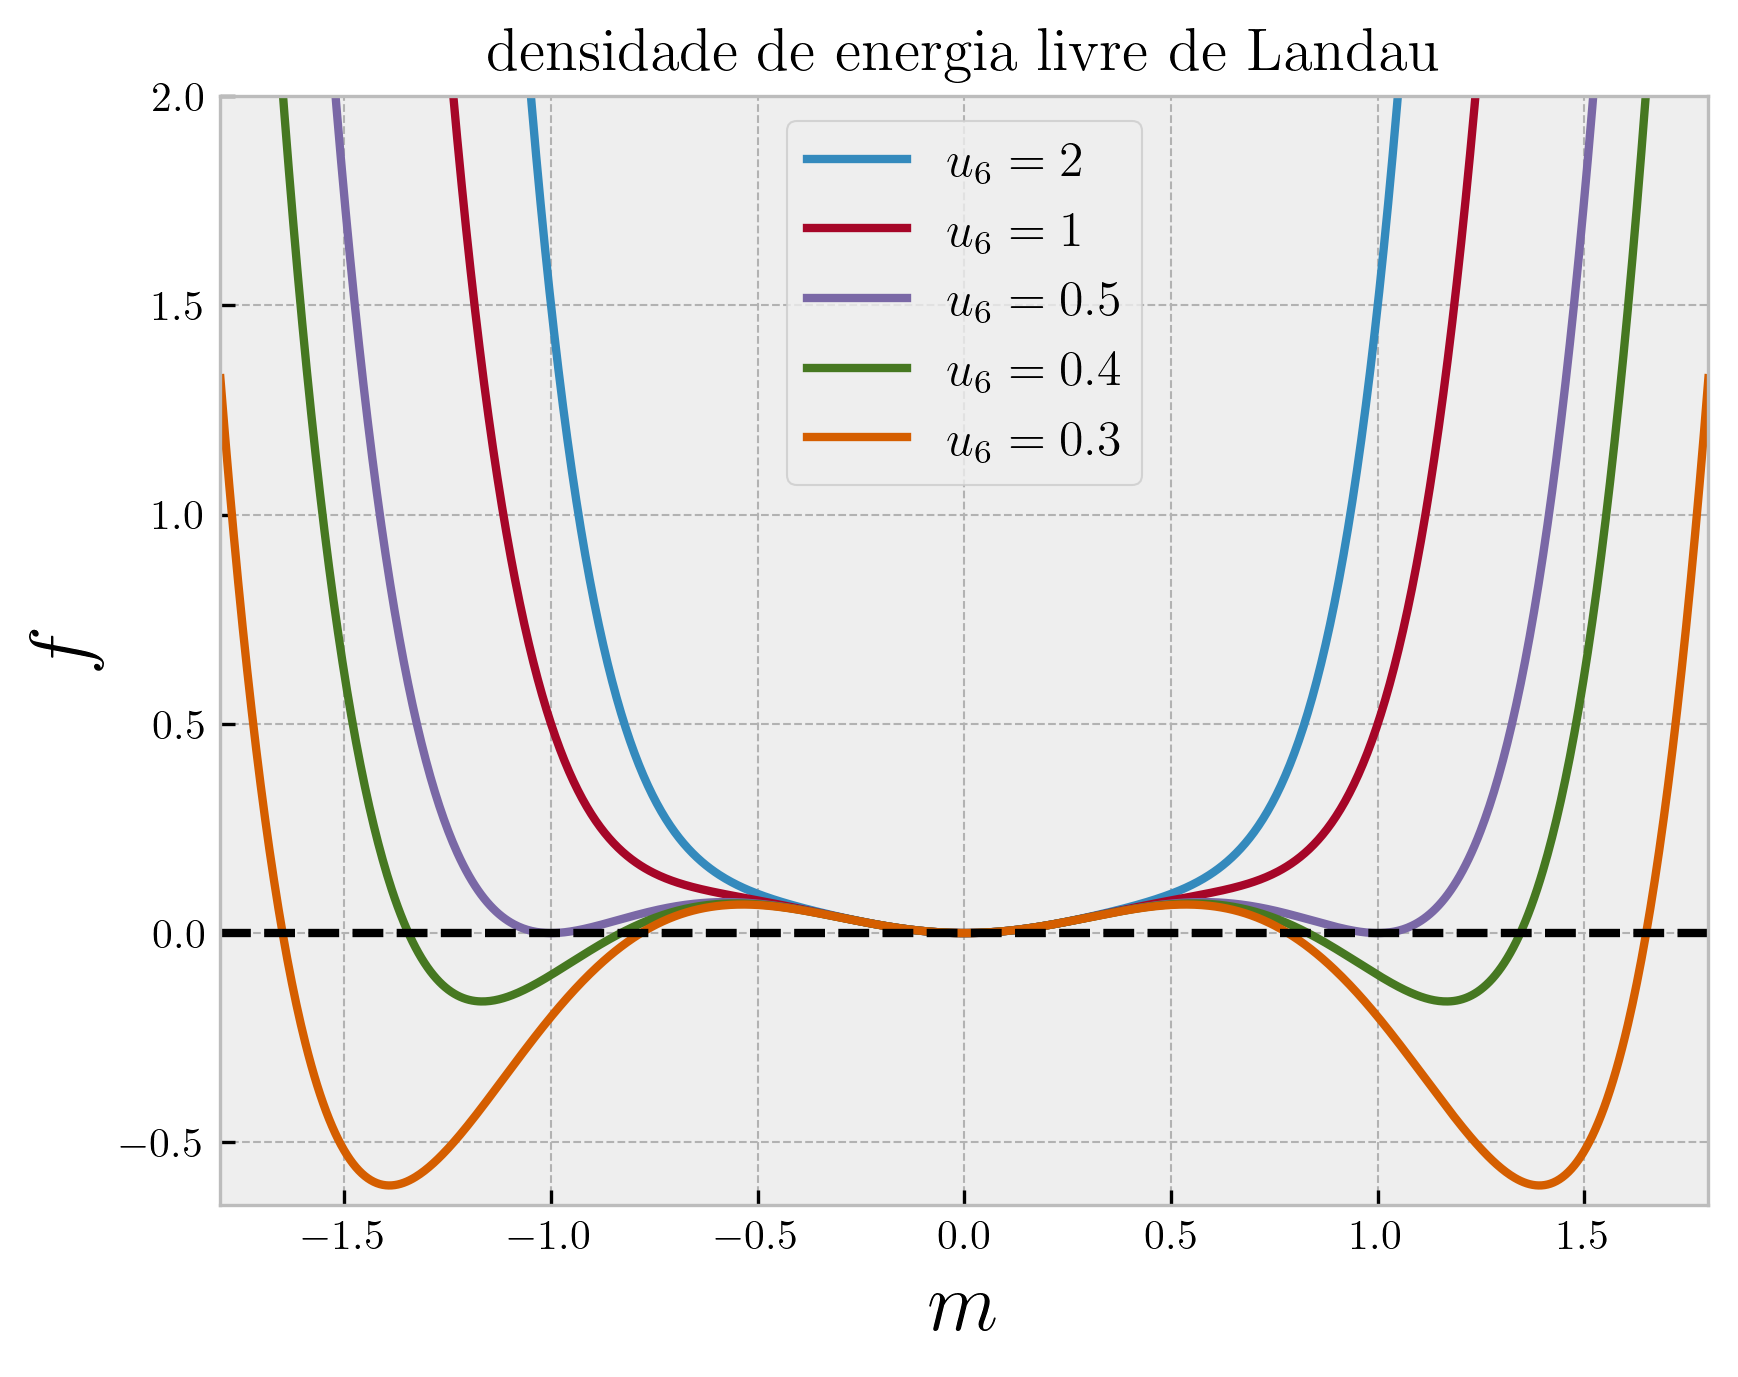
\includegraphics[width=0.6\linewidth]{fig/landau-free_energy.png}
\caption{Densidade de energia livre de Landau para $r = 1$, $u_4 = -1$ e diferentes valores de $u_6$.}
\label{fig:landau-free}
\end{figure}

Calculemos os mínimos locais de $f$:
\begin{itemize}
\item Caso $u_4 > 0$, em que podemos ignorar $u_6$.
$$
\pdv{f}{m} = m r + 4 u_4 m^3 = m (r + 4u_4 m^2) = 0.
$$

As soluções são $m = 0$ (trivial) e
$$
m_{\pm} = \pm\sqrt{-\frac{r}{4u_4}},
$$
que só existem quando $r < 0$. A segunda derivada é
$$
\pdv[2]{f}{m} = r + 12 u_4 m^2 \implies
\pdv[2]{f(0)}{m} = r \e \pdv[2]{f(m_{\pm})}{m} = -2r.
$$

Assim, a fase não-ordenada ($m=0$) é estável quando $r > 0$ e a fase ordenada ($m=m_\pm$) quando $r < 0$. Além disso, temos que
$$
f(m_\pm) = -\frac{r^2}{16 u_4} < 0 = f(0).
$$

Isso mostra que $r_c = 0$ para esse caso.


\item $u_4 < 0$.
$$
\pdv{f}{m} = m r + 4 u_4 m^3 + 6 u_6 m^5 = m (r + 4u_4 m^2 + 6 u_6 m^4) = 0.
$$
$$
\pdv[2]{f}{m} = r + 12 u_4 m^2 + 30 u_6 m^4.
$$

As raízes são $m = 0$ (trivial) e
$$
m_{\pm}^2 = \frac{- 4 u_4 \pm \sqrt{16 u_4^2 - 24 u_6 r}}{12 u_6},
$$
que só existem quando $u_4 < 0$. Somente alguma das duas soluções $m_+^2$ ou $m_-^2$ é um mínimo local, o outro é um máximo local. Utilizando o Mathematica, ele nos mostra que $\displaystyle{\pdv[2]{f(m_-)}{m}} < 0$ para quaisquer valores de $r > 0$ e $u_6 > 0$. Assim, a fase estável na verdade corresponde ao $m_+^2$.

\n

A transição ocorre quando a raiz $m_{+}$ possui uma energia livre menor que a da solução trivial $m = 0$ (que é $f(0) = 0$). Depois da transição para a fase ordenada temos
$$
f(m_+) < 0 = f(0).
$$
Podemos estudar essa inequação com a função \texttt{Reduce} do Mathematica:
$$
\texttt{Reduce}\qty[\Big\{r > 0, u_4 < 0, u_6 > 0, f(m_+) < 0\Big\},
\; \texttt{Reals}].
$$

O Mathematica nos retorna que $r$ deve satisfazer $r < \frac{u_4^2}{2 u_6} = r_c$. Isso mostra que temos a fase não-ordenada para $r > r_c$ e a fase ordenada para $r < r_c$.

\end{itemize}

Concluimos que
$$
r_c = a(T_c - T^*) =
\begin{cases}
\; 0, \quad & u_4 > 0, \\
\; \frac{u_4^2}{2 \abs{u_6}}, \quad & u_4 > 0.
\end{cases}
$$

\n

Podemos então resumir os resultados de nossos cálculos e montar o diagrama de fases $r-u_4$.
\begin{itemize}
\item Para $u_4 > 0$, temos a fase não-ordenada para $r > 0$ e ordenada para $r > 0$.
\item Para $u_4 < 0$, temos a fase não-ordenada para $r > \frac{u_4^2}{2 \abs{u_6}}$ e ordenada para $r < \frac{u_4^2}{2 \abs{u_6}}$.
\end{itemize}

O diagrama de fases é mostrado na Figura \ref{fig:phase_diag-tricrit}. O ponto $(r,u_4) = (0,0)$ é tricrítico pois temos 3 linhas contínuas (em verde claro na Figura \ref{fig:phase_diag-tricrit}) que se encontram em $(0,0)$.
\begin{figure}[H]
\centering
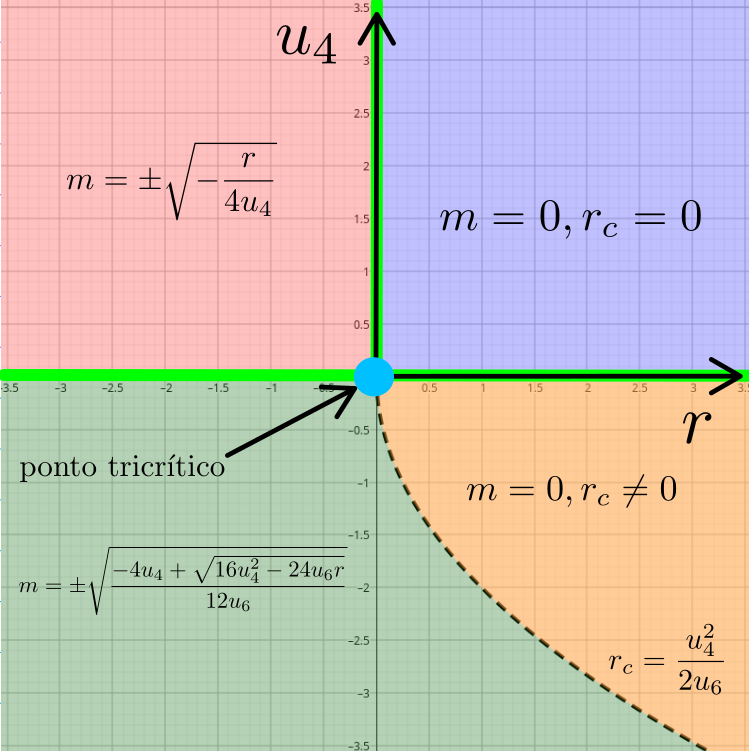
\includegraphics[width=0.49\linewidth]{fig/phase_diag-tricrit.png}
\caption{Diagrama de fases $r - u_4$. As linhas sólidas verdes indicam transições contínuas enquanto que a linha tracejada preta indica uma transição descontínua.}
\label{fig:phase_diag-tricrit}
\end{figure}

(b) As três linhas verdes na Figura \ref{fig:phase_diag-tricrit} são contínuas pois $m$ e $r$ passam por zero continuamente na transição. Agora, a linha tracejada preta é descontínua pois o valor de $m = 0$ (na fase não-ordenada) muda abruptamente na fase ordenada para
$$
m_+(r = r_c) = \pm\sqrt{\frac{- 4 u_4 + \sqrt{16 u_4^2 - 24 u_6 \qty(\frac{\abs{u_4}^2}{2 u_6})}}{12 u_6}} = \pm\sqrt{\frac{\abs{u_4}}{2 u_6}}.
$$

\n

Temos que
$$
s = - \pdv{f}{T} = -\frac{1}{2 T_c} a m_c^2 = -\frac{a}{4 T_c} \, \frac{u_4}{u_6},
$$
de maneira que o calor latente é
$$
q = - T_c \, s = \frac{a u_4}{4 u_6}.
$$

\n

Assumiremos agora que $u_4 = 0$ e calcularemos os expoentes críticos $\beta$, $\delta$ e $\gamma$. A densidade de energia livre e sua derivada são
$$
f = \frac{1}{2} rm^2 + u_6 m^6 - h m,
$$
$$
\pdv{f}{m} = rm + 6 u_6 m^5 - h.
$$

\n

Temos então
$$
\eval{\pdv{f}{m}}_{h=0} = rm + 6 u_6 m^5 = 0 \implies m = \qty(-\frac{r}{6u_6})^{1/4} \propto (T_c - T)^{1/4},
$$
de maneira que $\beta = 1/4$.

\n

Para $T \to T_c$ temos $r \to 0$ e
$$
\eval{\pdv{f}{m}}_{T_c} = 6 u_6 m^5 - h = 0 \implies m = \qty(\frac{h}{6u_6})^{1/5} \propto h^{1/5},
$$
que mostra que $\delta = 5$.

\n

Derivando com respeito a $h$ e fazendo $T \to T_c$ ($m \to 0$) e $h \to 0$, temos
$$
\pdv{f}{m} = rm + 6 u_6 m^5 - h = 0 \implies r \chi + 30 u_6 m^4 \chi - 1 = 0 \implies
\chi = \frac{1}{r + 30 u_6 m^4} \approx \frac{1}{r} \propto t^{-1},
$$
de maneira que o último expoente é $\gamma = 1$.



\pagebreak

\section*{5) Parâmetros de ordem acoplados}

Temos
$$
f = \frac{1}{2} r_1 m_1^2 + \frac{1}{2} r_2 m_2^2 + u_1 m_1^4 + u_2 m_2^4 + 2 u_{12} m_1^2 m_2^2,
$$
onde $u_1$, $u_2$ e $u_{12}$ são positivos. Defina $\boxed{\Delta = u_1 u_2 - u_{12}^2}$. No item (a) devemos estudar o diagrama de fases para $\Delta > 0$ e no item (b) para $\Delta < 0$.

\n

Pelas definições $r_1 = r - g = a(T-T_1)$ e $r_2 = r+g = a(T-T_2)$, observe que
$$
\begin{cases}
\; g > 0 \iff T_1 > T_2, \\
\; g < 0 \iff T_1 < T_2, \\
\; r_1 < 0 \iff g < r \iff T < T_1, \\
\; r_2 < 0 \iff g > -r \iff T < T_2.
\end{cases}
$$


As fases são caracterizadas por mínimos locais da função $f(m_1, m_2)$. Logo, para estudá-las devemos analisar os pontos em que $\grad{f} = \0$ e que o hessiano de $f$ seja \textit{positivo-definido} (é uma matriz simétrica com autovalores estritamente positivos).

\n

No caso particular de uma matriz simétrica $A$ de dimensão $2 \times 2$, ser positiva-definida significa que
$$
A =
\begin{pmatrix}
A_{11} & A_{12} \\
A_{12}& A_{22}
\end{pmatrix}
, \quad A_{11} > 0, \; A_{22} > 0 \; \text{ e } \det(A) = A_{11} A_{22} - A_{12}^2 > 0.
$$

O gradiente de $f$ é
$$
\grad{f} = \qty(\pdv{f}{m_1}, \pdv{f}{m_2}) =
\qty(r_1 m_1 + 4u_1 m_1^3 + 4u_{12} m_1 m_2^2, \; r_2 m_2 + 4u_2 m_2^3 + 4u_{12} m_2 m_1^2).
$$

Enquanto isso, o hessiano de $f$ é
$$
H_f(x, y) =
\begin{pmatrix}
\pdv[2]{f}{m_1} & \pdv{f}{m_1}{m_2} \\
\pdv{f}{m_2}{m_1} & \pdv[2]{f}{m_2}
\end{pmatrix}
=
\begin{pmatrix}
r_1 + 12 u_1 m_1^2 + 4 u_{12} m_2^2  & 8 u_{12} m_1 m_2 \\
8 u_{12} m_1 m_2 & r_2 + 12 u_2 m_2^2 + 4 u_{12} m_1^2
\end{pmatrix}.
$$


Igualando o gradiente a zero, temos
$$
\boxed{m_1 \Big(
r_1 + 4 u_1 m_1^2 + 4 u_{12} m_2^2
\Big) = 0,}
$$
$$
\boxed{m_2 \Big(
r_2 + 4 u_2 m_2^2 + 4 u_{12} m_1^2
\Big) = 0.}
$$

\n\n\n

As duas equações acima nos dão quatro possibilidades:
\begin{enumerate}
\item $m_1 = m_2 = 0$. Chamaremos esta fase de não-ordenada ($N$). Nela, o hessiano é
$$
H_f(0, 0) =
\begin{pmatrix}
r_1 & 0 \\
0 & r_2
\end{pmatrix}.
$$

Ele é positivo-definido para
$$
r_1 > 0 \e r_2 > 0 \implies \boxed{g < r \e g > -r.}
$$



\item $m_2 = 0$ e $m_1 = m^0_1 = \pm\sqrt{-\frac{r_1}{4 u_1}}$. Chamaremos esta fase de $(F_1)$, onde apenas $m_1 \neq 0$. Devido à raiz quadrada, note que ela só existe caso $r_1 < 0$. Durante a transição, $r_1$ muda de sinal positivo para negativo. Note então que a linha de transição de $(F_1)$ é contínua, já que $m_1 \propto \sqrt{-r_1}$. Calculando o hessiano nesta fase, obtemos
$$
H_f(m_1^0, 0) =
\begin{pmatrix}
-2 r_1 & 0 \\
0 & r_2 - \frac{u_{12}}{u_1} r_1
\end{pmatrix}.
$$

As condições de existência ($m_1$ e $m_2$ serem reais) e estabilidade (o hessiano ser positivo-definido) se traduzem como
$$
r_1 < 0 \e r_2 > \frac{u_{12}}{u_1} r_1
\implies
\boxed{g > r \e g > -\qty(\frac{u_1 - u_{12}}{u_1 + u_{12}}) r. }
$$



\item $m_1 = 0$ e $m_2 = m^0_2 = \pm\sqrt{-\frac{r_2}{4 u_2}}$. Chamaremos esta fase de $(F_2)$, onde apenas $m_2 \neq 0$. Devido à raiz quadrada, note que ela só existe caso $r_2 < 0$. Durante a transição, $r_2$ também muda de sinal positivo para negativo. Note então que a linha de transição de $(F_2)$ é contínua, já que $m_2 \propto \sqrt{-r_2}$. Calculando o hessiano, obtemos
$$
H_f(0, m_2^0) =
\begin{pmatrix}
r_1 - \frac{u_{12}}{u_2} r_2 & 0 \\
0 & -2 r_2
\end{pmatrix}.
$$

As condições de existência e estabilidade se traduzem como
$$
r_2 < 0 \e r_1 > \frac{u_{12}}{u_2} r_2
\implies
\boxed{g < -r \e g < \qty(\frac{u_{2} - u_{12}}{u_2 + u_{12}}) r. }
$$





\item $m_1 \neq 0$ e $m_2 \neq 0$. Chamaremos esta fase de ($F_{12}$). Descobrindo os valores de $m_1$ e $m_2$:
$$
\begin{cases}
\; r_1 + 4 u_1 m_1^2 + 4 u_{12} m_2^2 = 0 \quad [\times (u_{12})] \\
\; r_2 + 4 u_2 m_2^2 + 4 u_{12} m_1^2 = 0 \quad [\times (-u_{1})]
\end{cases}
\implies
\begin{cases}
\; + (u_{12} r_1 + \cancel{4 u_1 u_{12} m_1^2} + 4 u_{12}^2 m_2^2) = 0 \\
\; - (u_1 r_2 + 4 u_1 u_2 m_2^2 + \cancel{4 u_1 u_{12} m_1^2}) = 0
\end{cases}
\implies
$$
$$
(u_{12} r_1 - u_1 r_2) + 4 (u_{12}^2 - u_1 u_2) m_2^2 = 0 \implies
\boxed{ m_2^2 = \gamma_2 = \frac{u_{12} r_1 - u_1 r_2}{4 (u_1 u_2 - u_{12}^2)}, }
$$
e de maneira análoga
$$
\boxed{ m_1^2 = \gamma_1 = \frac{u_{12} r_2 - u_2 r_1}{4 (u_1 u_2 - u_{12}^2)}. }
$$

Perceba que esta fase $(F_{12})$ só existe caso as raízes quadradas sejam reais, ou seja, $\gamma_1 > 0$ e $\gamma_2 > 0$.


Calculando no Mathematica o hessiano da fase $(F_{12})$, temos
$$
H = H_f(\sqrt{\gamma_1}, \sqrt{\gamma_2}) =
\begin{pmatrix}
\frac{2 (u_{12} r_2 - u_2 r_1) u_1}{u_1 u_2 - u_{12}^2} &
2 u_{12} \sqrt{\frac{(u_{12} r_2 - u_2 r_1)(u_{12} r_1 - u_1 r_2))}{(u_{12}^2 - u_1 u_2)^2}} \\
2 u_{12} \sqrt{\frac{(u_{12} r_2 - u_2 r_1)(u_{12} r_1 - u_1 r_2))}{(u_{12}^2 - u_1 u_2)^2}} &
\frac{2 (u_{12} r_1 - u_1 r_2) u_2}{u_1 u_2 - u_{12}^2}
\end{pmatrix}.
$$

A fase $(F_{12})$ é estável se o hessiano $H$ for positivo-definido, ou seja, $H_{11}>0$, $H_{22}>0$ e $\det(H)>0$.

Utilizando as condições de existência e estabilidade da fase $(F_{12})$, a função \texttt{Reduce} do Mathematica simplifica todas as inequações. Eu inseri no Mathematica:
$$
\texttt{Reduce}\qty[\Big\{u_1 > 0, u_2 > 0, u_{12} > 0, \gamma_1 > 0, \gamma_2 > 0,
H_{11} > 0, H_{22} > 0, \det(H) > 0\Big\},
\; \texttt{Reals}].
$$

O Mathematica retornou
$$
\boxed{\Delta = u_1 u_2 - u_{12}^2 > 0}, \quad
r_2 < 0, \quad
r_1 < 0, \quad
r_2 < \frac{u_{12}}{u_1} r_1 \e
r_1 < \frac{u_{12}}{u_2} r_2.
$$

Em particular, isso mostra que a fase $(F_{12})$ só existe para $u_1 u_2 > u_{12}^2$. As condições para $r_1$ e $r_2$ se traduzem nas condições para $r$ e $g$:

$$
\boxed{
g > r, \quad
g < -r, \quad
g < -\qty(\frac{u_1 - u_{12}}{u_1 + u_{12}}) r \e
g > \qty(\frac{u_2 - u_{12}}{u_2 + u_{12}}) r. }
$$

Durante a transição, nós temos que $(u_{12} r_1 - u_1 r_2) \to 0^+$ ou que $(u_{12} r_2 - u_2 r_1) \to 0^+$. Como
$m_1 \propto \sqrt{u_{12} r_2 - u_2 r_1}$ e $m_2 \propto \sqrt{u_{12} r_1 - u_1 r_2}$, temos que as linhas de transição de $(F_{12})$ também são contínuas.


\end{enumerate}

(a) Usando os parâmetros $u_1 = 2$, $u_2 = 2$ e $u_{12} = 1$, que satisfazem a condição $\Delta = u_1 u_2 - u_{12}^2 > 0$ para a fase mista $(F_{12})$ existir, obtemos o seguinte diagrama de fase $r-g$ na Figura \ref{fig:phase_diag-tetra} (graficado no \href{https://www.desmos.com/calculator?lang=pt-BR}{Desmos}, onde inseri todas as inequações obtidas).
\begin{figure}[H]
\centering
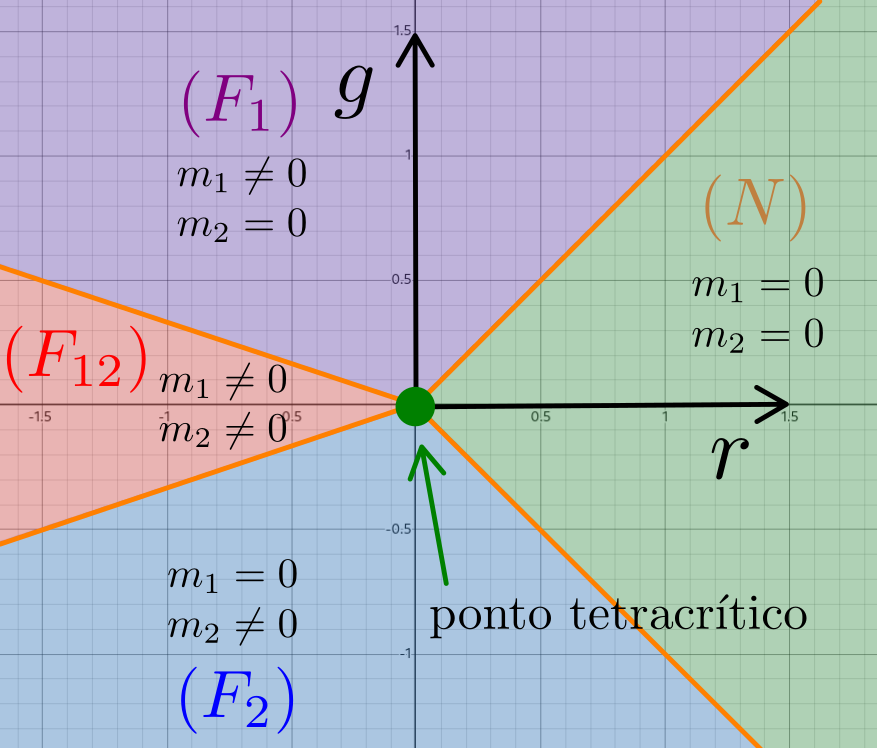
\includegraphics[width=0.4\linewidth]{fig/phase_diag-tetra.png}
\caption{Diagrama de fase para $u_1 = u_2 = 2$ e $u_{12} = 1$, situação em que existe a fase mista $(F_{12})$. As linhas de transição (\textcolor{Orange}{em laranja}) são contínuas e se encontram no ponto tetracrítico $(r = 0, g = 0)$.}
\label{fig:phase_diag-tetra}
\end{figure}

\n\n

(b) Neste item exploraremos o caso $u_1 u_2 < u_{12}^2$. Como fizemos cálculos gerais dos mínimos locais anteriormente, eles também valem aqui. Só que nesse caso a fase mista $(F_{12})$ não existe. As outras três fases $(N)$, $(F_1)$ e $(F_2)$ continuam a existir e são estáveis nas mesmas condições calculadas anteriomente. Se graficarmos o diagrama de fases (para mínimos locais), para os parâmetros $u_1 = 1/2$, $u_2 = 1/2$ e $u_{12} = 1$, obtemos a Figura \ref{fig:phase_diag-tri}.
\begin{figure}[H]
\centering
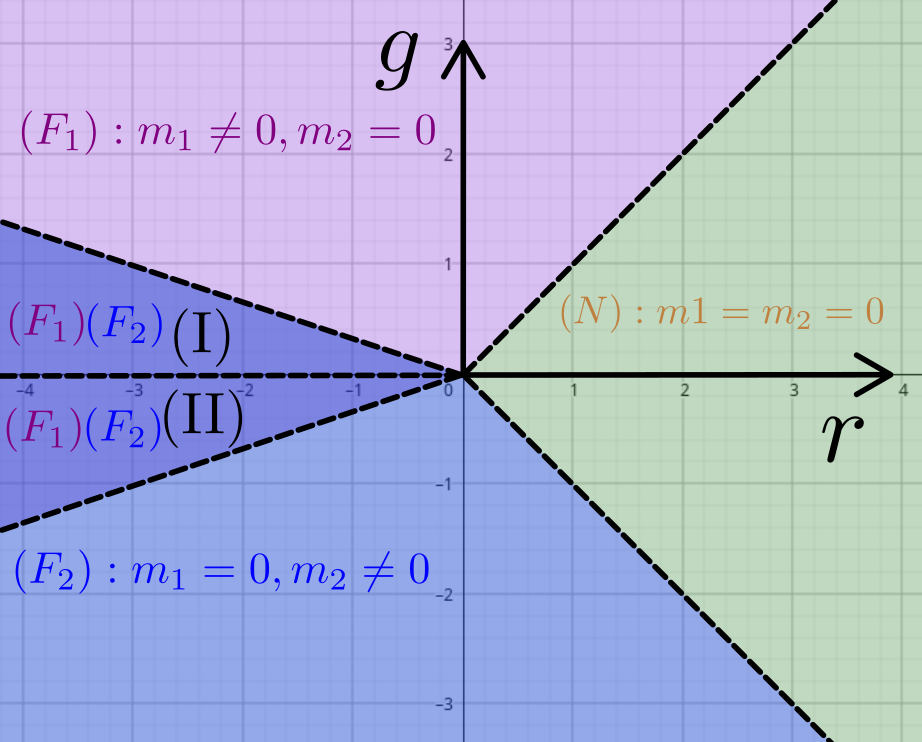
\includegraphics[width=0.4\linewidth]{fig/phase_diag-tri.png}
\caption{Diagrama de fases (mínimos locais) para $u_1 = 0.5$, $u_2 = 0.5$ e $u_{12} = 1$ ($u_1 u_2 < u_{12}^2$). Nesse caso, ambas as fases $(F_1)$ e $(F_2)$ coexistem e são estáveis nas regiões (I) e (II) destacadas à esquerda no gráfico. Mas somente uma delas é o mínimo global.}
\label{fig:phase_diag-tri}
\end{figure}

A explicação para ambas as fases $(F_1)$ e $(F_2)$ coexistirem estavelmente é que ambas se caracterizam como mínimos locais. Para descobrirmos qual fase \textbf{tem preferência}, basta calcularmos qual delas se configura como \textbf{mínimo global}.

\n

Faremos isso comparando $f_1 = f(m_1^0, 0)$ com $f_2 = f(0, m_2^0)$. Temos
$$
f_1 = f(m_1^0, 0) = - \frac{r_1^2}{16 u_1} < 0 \e
f_2 = f(0, m_2^0) = - \frac{r_2^2}{16 u_2} < 0.
$$

Assim, na região (I) da Figura \ref{fig:phase_diag-tri} (que satisfaz as condições $g > 0 \iff r_2 > r_1$ e $r_1 > \frac{u_{12}}{u_2} r_2$), temos
$$
f_1 = - \frac{r_1^2}{16 u_1} < -\frac{u_{12}^2 r_2^2}{16 u_1 u_2^2} = \frac{u_{12}^2}{u_1 u_2}\qty(-\frac{r_2^2}{16 u_2}) = \frac{u_{12}^2}{u_1 u_2} \, f_2 < f_2 \implies \boxed{f_1 < f_2.}
$$

Isso mostra que na região (I) a fase $(F_1)$ tem preferência. Analogamente mostra-se que na região (II) a fase $(F_2)$ tem preferência.

\n

Da mesma forma que no item (a), as transições para a região $(N)$ são contínuas.

\n

Agora, a transição entre as duas fases $(F_1)$ e $(F_2)$ é descontínua, porque mesmo para $r_1$ longe de zero, a fase $(F_1)$ tem $m_1^2 = -\frac{r_1}{4u_1}$, que pula abruptamente para $m_1 = 0$ quando há transição para a fase $(F_2)$. O análogo acontece com $m_2$.

\n


\n\n

O diagrama de fases é então exibido na Figura \ref{fig:phase_diag-bi}.
\begin{figure}[H]
\centering
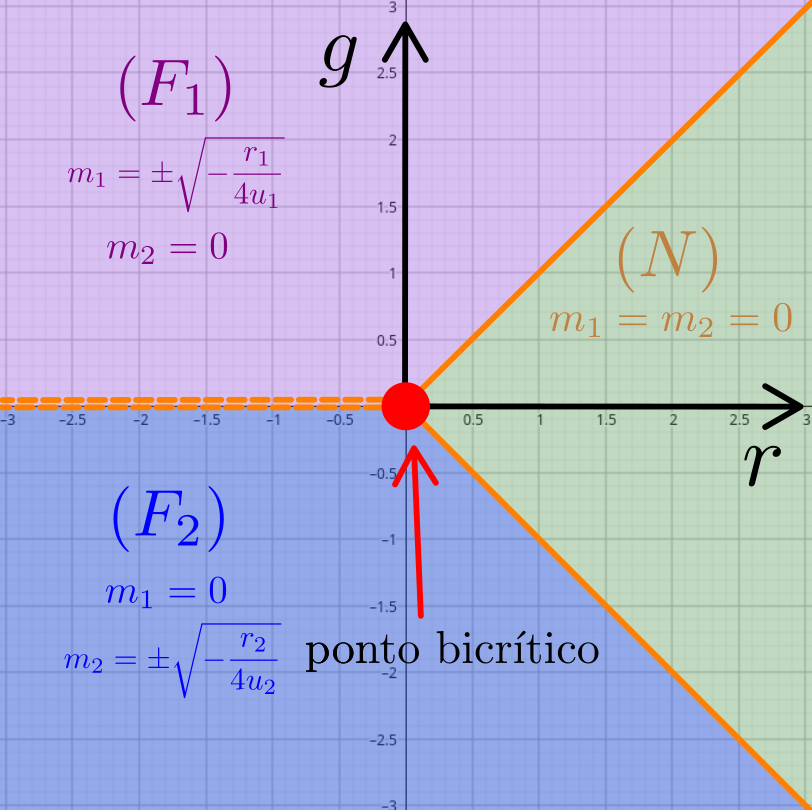
\includegraphics[width=0.6\linewidth]{fig/phase_diag-bi.png}
\caption{Diagrama de fases (mínimos globais) para $u_1 u_2 < u_{12}^2$. As linhas sólidas laranjas são contínuas, enquanto que a linha dupla tracejada laranja configura uma transição descontínua.}
\label{fig:phase_diag-bi}
\end{figure}

\n\n

No caso em que $u_{12} < 0$ e $u_{12}^2 > u_1 u_2$, existem valores de $m_1$ e $m_2$ para os quais a energia livre $f(m_1, m_2)$ decresce indefinidamente. Por exemplo, se $u_1 = 1$, $u_2 = 1$ e $u_{12} = -2$, podemos tomar $m_1 = m_2 = m \to \infty$, de maneira que $f \to -\infty$. Isso se configura como uma região instável, que não faz sentido físico, pois as magnetizações $m_1$ e $m_2$ crescem indefinidamente.


%%%-----
%%% Referências bibliográficas
%%%-----
%\addcontentsline{toc}{chapter}{\bibname}
%%\bibliographystyle{abntex2-num}
%\bibliography{citations}
%\bibliographystyle{ieeetr}


\end{document}
